\documentclass[12pt]{article}

\usepackage{blindtext}
\usepackage[hidelinks]{hyperref}

\usepackage{subcaption}
\usepackage{graphicx}
\usepackage{xcolor}
\usepackage{amsmath}
\usepackage{amsfonts}
\usepackage{caption}
\usepackage{subcaption}




\title{\textbf{Histogram Equalization}}
\author{\href{https://github.com/rezaAdinepour/Histogram-Equalization.git}{\textcolor{blue}{Reza Adinepour}}}



\begin{document}
	
\maketitle
Histogram equalization is a basic image processing technique that adjusts the global contrast of an image by updating the image histogram’s pixel intensity distribution. Doing so enables areas of low contrast to obtain higher contrast in the output image.

Essentially, histogram equalization works by:
\begin{enumerate}
	\item Computing a histogram of image pixel intensities
	\item  Evenly spreading out and distributing the most frequent pixel values (i.e., the ones with the largest counts in the histogram)
	\item Giving a linear trend to the cumulative distribution function (CDF)
\end{enumerate}

The result of applying histogram equalization is an image with higher global contrast.

We can further improve histogram equalization by applying an algorithm called Contrast Limited Adaptive Histogram Equalization (CLAHE), resulting in higher quality output images.

Other than photographers using histogram equalization to correct under/overexposed images, the most widely used histogram equalization application can be found in the medical field.

You’ll typically see histogram equalization applied to X-ray scans and CT scans to improve the radiograph’s contrast. Doing so helps doctors and radiologists better interpret the scans and make an accurate diagnosis.

By the end of this tutorial, you will be able to successfully apply both basic histogram equalization and adaptive histogram equalization to images with OpenCV.


\section{Theoretical definitions}
	\subsection{Image}
	A digital image is a discrete space composed of small surface elements called pixel. Each one of this elements contains a value or a set of value coding the intensity level at each position. A digital image can be acquired with a great number of different devices such as a camera, an MRI machine or any kind of device with a sensor able to capture light intensity.
	
	Because of its discrete nature, the theory used to process digital image will rely on discrete domain, even if the analogy with the continuous domain is possible.
	
	\begin{itemize}
		\item \textbf{Gray scale digital image}
		
		A gray scale image is a digital image in which each pixel only contains one scalar value which is its intensity. The number of possible levels (intensity values) depends on the numerical type encoding the image.
		
		For example, an image encoded with $n=8$ bits will only have $L=28=256$ possible intensity values going from 0 representing black to $L-1=255$ representing white.
		
		\item \textbf{Color image}
		
		A color image is a digital array of pixel containing a color information. Each image can be decomposed into three different layers according to the three color channels encoded: Red, Green and Blue.
		
		For instance, a $8$ bits color images encode the Red and Green channel with three bits and the blue with two. Which could encode $256$ different colors.
	\end{itemize}

	\subsection{Histogram}
	The histogram of a digital image is a distribution of its discrete intensity levels in the range $[0, L-1]$. The distribution is a discrete function h associating to each intensity level: $r_k$ the number of pixel with this intensity: $n_k$.
	
	\subsection{Transformation of Histogram}
	\begin{itemize}
		\item \textbf{Normalization of a Histogram}
		
		Normalize an histogram is a technique consisting into transforming the discrete distribution of intensities into a discrete distribution of probabilities. To do so, we need to divide each value of the histogram by the number of pixel. Because a digital image is a discrete set of values that could be seen as a matrix and it's equivalent to divide each $n_k$ by the dimension of the array which is the product of the width by the length of the image.
		
		\begin{equation}
			n_{kn} = \frac{n_k}{length \times width} = p_{r}(r_k)
		\end{equation}
		
		Which could be written in terms of mathematical transformation:
		\begin{equation}
			\begin{cases}
				[0, L-1] \rightarrow \mathbb{N} \\
				x \rightarrow Card(x) 
			\end{cases}
		\end{equation}
		\begin{equation}
			becomes \begin{cases}
				[0, L-1] \rightarrow [0, 1] \\
				x \rightarrow pdf(x) = \frac{Card(x)}{\sum_{i=0}^{L-1} Card(x_i)}
			\end{cases}
		\end{equation}
	
		Where Card means the cardinality of the set so in our case the number of pixel.
		
		\item \textbf{Equalization of a Histogram}
		
		Histogram equalization is a method to process images in order to adjust the contrast of an image by modifying the intensity distribution of the histogram. The objective of this technique is to give a linear trend to the cumulative probability function associated to the image.
		
		The processing of histogram equalization relies on the use of the cumulative probability function (cdf). The cdf is a cumulative sum of all the probabilities lying in its domain and defined by:
		\begin{equation}
			cdf(x) = \sum_{k=-\infty}^{x} P(k)
		\end{equation}
		
		The idea of this processing is to give to the resulting image a linear cumulative distribution function. Indeed, a linear cdf is associated to the uniform histogram that we want the resulting image to have.
		
		\begin{figure}[h]
			\centering
			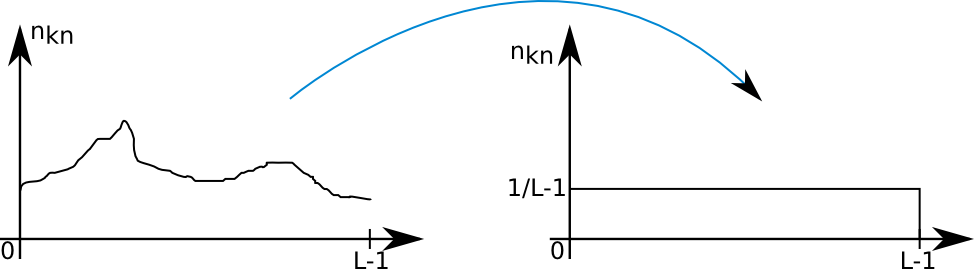
\includegraphics[width=1\textwidth]{images/2}
			\caption{Technique to perform histogram equalization}
			\label{fig:fig1}
		\end{figure}
		
		So we are going to implement the following formula to get the new pdf:
		\begin{equation}
			S_k = (L - 1)cdf(x)
		\end{equation}
	
		\item Segmentation with an histogram
		
		Segmentation is an operation consisting in partitioning an image into sets of elements. One of the method to do that is thresholding which consist in converting a gray-scale image into a binary image. The most important step here is to chose the best value for the threshold to get the best segmentation. Several methods exists to determine it.
		
		\begin{figure}[h]
			\centering
			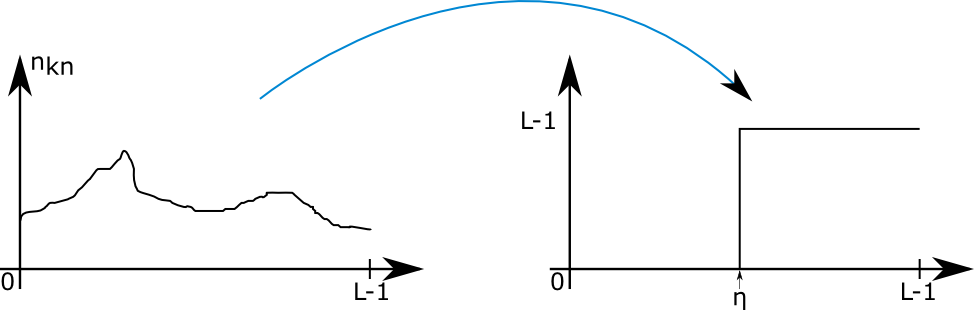
\includegraphics[width=1\textwidth]{images/3}
			\caption{Segmentation using a single threshold}
			\label{fig:fig2}
		\end{figure}
	\end{itemize}

	\subsection{Gaussian or Normal distribution}
	The Gaussian probability distribution function is a kind of pdf defined by:
	\begin{equation}
		\begin{cases}
			\mathbb{R} \rightarrow [0, 1]\\
			G_{1}(x) = \frac{1}{\sqrt{2\pi}\sigma}e^{\frac{-(x-\bar{m})^2}{2\sigma^2}}
		\end{cases}
	\end{equation}
	
	with:‌ $\bar{m}$ being the mean and $\sigma$ being the standard deviation
	
	\begin{figure}[h]
		\centering
		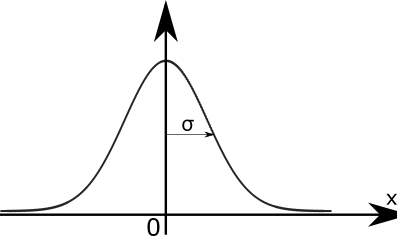
\includegraphics[width=.7\textwidth]{images/4}
		\caption{Gaussian distribution with 0 mean and a standard deviation}
		\label{fig:fig3}
	\end{figure}

\section{Programing}
For this project, all the programming to process images and create the results associated to each experiment is made with Python.

all the code I'm going to present here is using Python programing language syntax. But all algorithm will work with any other languages. A more detailed presentation of the code is available in my \href{https://github.com/rezaAdinepour/Histogram-Equalization.git}{\textcolor{magenta}{Github page}}.

All of data is available in \texttt{Images} folder. After you run the code, all the images  in the \texttt{Images} folder will be shown to you and you can select one of them.

\begin{figure}[h]
	\centering
	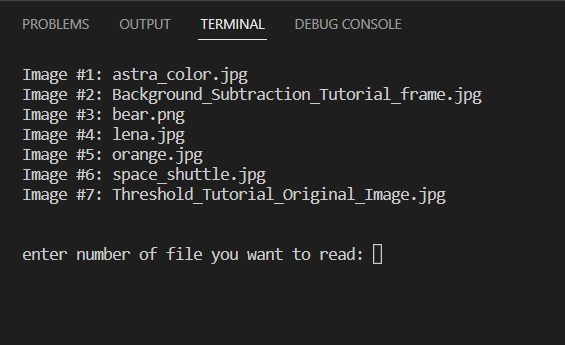
\includegraphics[width=.7\textwidth]{images/5}
	\caption{available data in \texttt{Images} folder}
	\label{fig:fig4}
\end{figure}

For example, I select \texttt{Image \#4: lena.jpg} and then we see the output of the algorithm:

\begin{figure}
	\centering
	\begin{subfigure}[b]{0.3\textwidth}
		\centering
		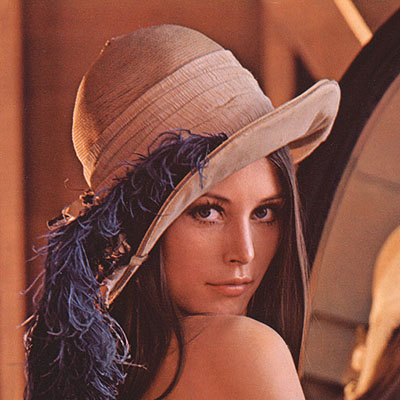
\includegraphics[width=\textwidth]{images/lena}
		\caption{Original image}
		\label{fig:org_lena}
	\end{subfigure}
	\hfill
	\begin{subfigure}[b]{0.3\textwidth}
		\centering
		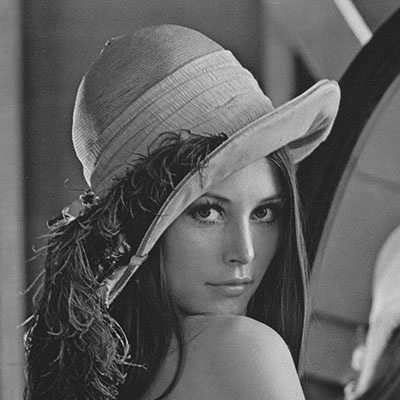
\includegraphics[width=\textwidth]{images/gray_lena}
		\caption{Gray scale image}
		\label{fig:gray_lena}
	\end{subfigure}
	\hfill
	\begin{subfigure}[b]{0.3\textwidth}
		\centering
		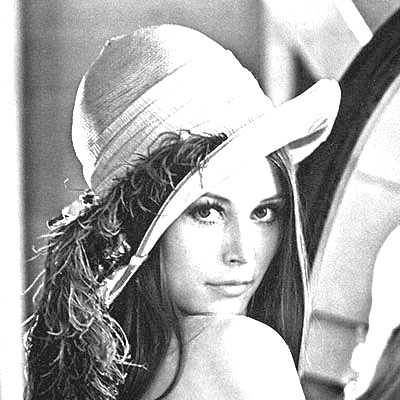
\includegraphics[width=\textwidth]{images/high_contrast_lena}
		\caption{High contrast image}
		\label{fig:lena_high}
	\end{subfigure}
	\caption{Output of \texttt{lena.jpg} image}
	\label{fig:lena}
\end{figure}

\begin{figure}[h]
	\centering
	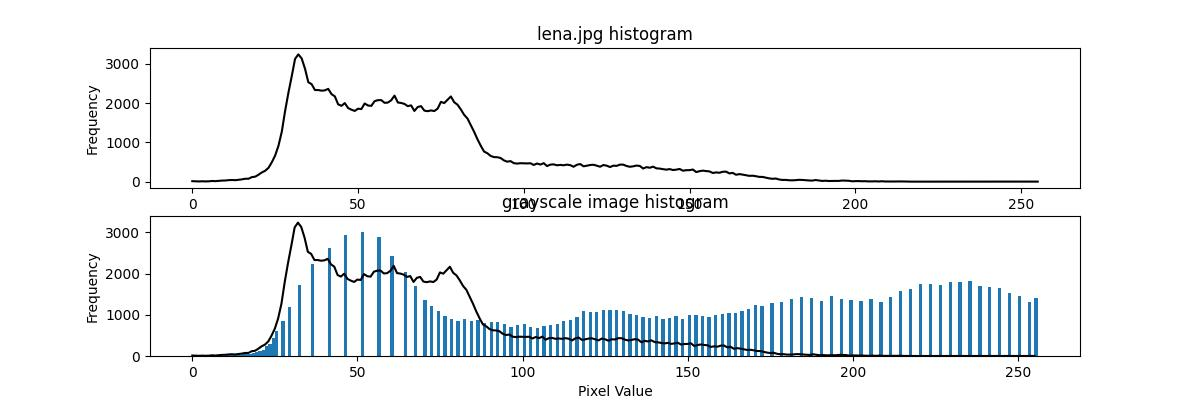
\includegraphics[width=1\textwidth]{images/fig_lena}
	\caption{\texttt{lena.jpg} histogram}
	\label{fig:lena_hist}
\end{figure}

For any question please send me an email:
\href{mailto:r3zaadinep0ur@gmail.com}{\textcolor{blue}{r3zaadinep0ur@gmail.com}}

\end{document}